\todo{Say something about more the collection of examples available online: }
The collection of examples is available in the \verb+examples/+ directory of the GitHub repository \href{https://github.com/GRACeFUL-project/GenericLibrary}{GenericLibrary}:

% -- A GCM representing a simluation of the swedish energy system
% energySystem :: GCM ()
% SmallExample.hs

\subsection{Example: Runoff flow}
\label{example-runoff-flow}

We show a small GL program which models a rain runoff area, like a
town square, which has been provided with a pump to alleviate possible
flooding issues (this is a common procedure in countries like the
Netherlands).
%
This example is a small part of a larger model used in the CRUD case
study meant to show how GL can be employed to model concrete problems
in CRUD.


\subsubsection{DSL textual input}
\label{example-runoff-flow-dsl-textual-input}

Here we show a complete example with three components.
%
Fig. \ref{fig:RunoffEx} shows a graphical view of how the components
are connected.
%
\begin{figure}[htbp]
  \centering
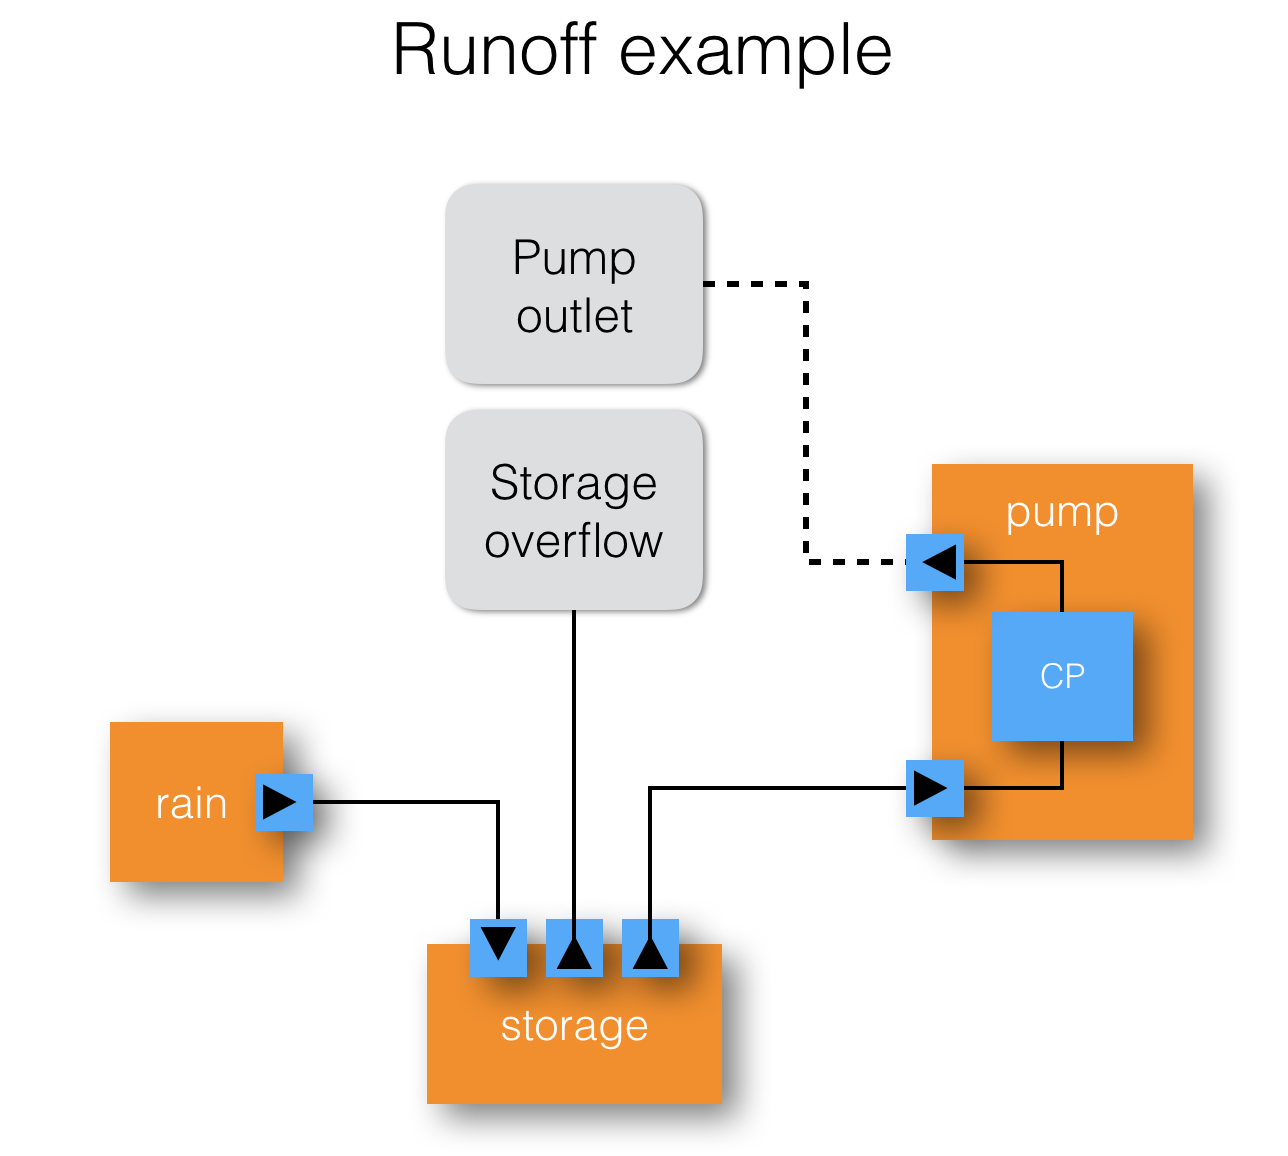
\includegraphics[width=0.5\textwidth]{fig/RunoffExample.jpg}
  \caption{Runoff example structure}
  \label{fig:RunoffEx}
\end{figure}

\begin{verbatim}
pump :: Float -> GCM (Port Float, Port Float)
pump ... -- As before

rain :: Float -> GCM (Port Float)
rain ... -- As before

storage :: Float -> GCM (Port Float, Port Float, Port Float)
storage cap = do
  inflow   <- createPort
  outlet   <- createPort
  overflow <- createPort
  component $ do
    currentStored <- createVariable
    inf <- value inflow
    out <- value outlet
    ovf <- value overflow
    sto <- value currentStored
    assert $ sto === inf - out - ovf
    assert $ sto `inRange` (0, lit cap)
    assert $ (ovf .> 0) ==> (sto === lit cap)
    assert $ ovf .>= 0
  return (inflow, outlet, overflow)

example :: GCM ()
example = do
  (inflowP, outflowP) <- pump 5
  (inflowS, outletS, overflowS) <- storage 4
  rainflow <- rain 10

  link inflowP outletS
  link inflowS rainflow

  output "Overflow" overflowS
\end{verbatim}

Our example is compiled and run using the \texttt{runGCM} command.
%
The constraint programming runtime, \texttt{MiniZinc}, informs us
that with the numbers in our example the overflow will be zero.

\begin{verbatim}
ghci> runGCM example
{"Overflow" : 0}
\end{verbatim}

While this example is easily calculated by hand GL is capable of
expressing more complicated, and less self-contained, GRACeFUL concept
maps including actions and optimization problems.
%
As these examples are somewhat larger we omit them in this document
and refer to the online resources mentioned earlier.
